% Options for packages loaded elsewhere
\PassOptionsToPackage{unicode}{hyperref}
\PassOptionsToPackage{hyphens}{url}
\PassOptionsToPackage{dvipsnames,svgnames,x11names}{xcolor}
%
\documentclass[
  12pt,
  a4paper,
]{article}
\usepackage{amsmath,amssymb}
\usepackage{lmodern}
\usepackage{setspace}
\usepackage{iftex}
\ifPDFTeX
  \usepackage[T1]{fontenc}
  \usepackage[utf8]{inputenc}
  \usepackage{textcomp} % provide euro and other symbols
\else % if luatex or xetex
  \usepackage{unicode-math}
  \defaultfontfeatures{Scale=MatchLowercase}
  \defaultfontfeatures[\rmfamily]{Ligatures=TeX,Scale=1}
\fi
% Use upquote if available, for straight quotes in verbatim environments
\IfFileExists{upquote.sty}{\usepackage{upquote}}{}
\IfFileExists{microtype.sty}{% use microtype if available
  \usepackage[]{microtype}
  \UseMicrotypeSet[protrusion]{basicmath} % disable protrusion for tt fonts
}{}
\makeatletter
\@ifundefined{KOMAClassName}{% if non-KOMA class
  \IfFileExists{parskip.sty}{%
    \usepackage{parskip}
  }{% else
    \setlength{\parindent}{0pt}
    \setlength{\parskip}{6pt plus 2pt minus 1pt}}
}{% if KOMA class
  \KOMAoptions{parskip=half}}
\makeatother
\usepackage{xcolor}
\usepackage[left=2.54cm,right=2.54cm,top=2.54cm,bottom=2.54cm]{geometry}
\usepackage{color}
\usepackage{fancyvrb}
\newcommand{\VerbBar}{|}
\newcommand{\VERB}{\Verb[commandchars=\\\{\}]}
\DefineVerbatimEnvironment{Highlighting}{Verbatim}{commandchars=\\\{\}}
% Add ',fontsize=\small' for more characters per line
\usepackage{framed}
\definecolor{shadecolor}{RGB}{248,248,248}
\newenvironment{Shaded}{\begin{snugshade}}{\end{snugshade}}
\newcommand{\AlertTok}[1]{\textcolor[rgb]{0.94,0.16,0.16}{#1}}
\newcommand{\AnnotationTok}[1]{\textcolor[rgb]{0.56,0.35,0.01}{\textbf{\textit{#1}}}}
\newcommand{\AttributeTok}[1]{\textcolor[rgb]{0.77,0.63,0.00}{#1}}
\newcommand{\BaseNTok}[1]{\textcolor[rgb]{0.00,0.00,0.81}{#1}}
\newcommand{\BuiltInTok}[1]{#1}
\newcommand{\CharTok}[1]{\textcolor[rgb]{0.31,0.60,0.02}{#1}}
\newcommand{\CommentTok}[1]{\textcolor[rgb]{0.56,0.35,0.01}{\textit{#1}}}
\newcommand{\CommentVarTok}[1]{\textcolor[rgb]{0.56,0.35,0.01}{\textbf{\textit{#1}}}}
\newcommand{\ConstantTok}[1]{\textcolor[rgb]{0.00,0.00,0.00}{#1}}
\newcommand{\ControlFlowTok}[1]{\textcolor[rgb]{0.13,0.29,0.53}{\textbf{#1}}}
\newcommand{\DataTypeTok}[1]{\textcolor[rgb]{0.13,0.29,0.53}{#1}}
\newcommand{\DecValTok}[1]{\textcolor[rgb]{0.00,0.00,0.81}{#1}}
\newcommand{\DocumentationTok}[1]{\textcolor[rgb]{0.56,0.35,0.01}{\textbf{\textit{#1}}}}
\newcommand{\ErrorTok}[1]{\textcolor[rgb]{0.64,0.00,0.00}{\textbf{#1}}}
\newcommand{\ExtensionTok}[1]{#1}
\newcommand{\FloatTok}[1]{\textcolor[rgb]{0.00,0.00,0.81}{#1}}
\newcommand{\FunctionTok}[1]{\textcolor[rgb]{0.00,0.00,0.00}{#1}}
\newcommand{\ImportTok}[1]{#1}
\newcommand{\InformationTok}[1]{\textcolor[rgb]{0.56,0.35,0.01}{\textbf{\textit{#1}}}}
\newcommand{\KeywordTok}[1]{\textcolor[rgb]{0.13,0.29,0.53}{\textbf{#1}}}
\newcommand{\NormalTok}[1]{#1}
\newcommand{\OperatorTok}[1]{\textcolor[rgb]{0.81,0.36,0.00}{\textbf{#1}}}
\newcommand{\OtherTok}[1]{\textcolor[rgb]{0.56,0.35,0.01}{#1}}
\newcommand{\PreprocessorTok}[1]{\textcolor[rgb]{0.56,0.35,0.01}{\textit{#1}}}
\newcommand{\RegionMarkerTok}[1]{#1}
\newcommand{\SpecialCharTok}[1]{\textcolor[rgb]{0.00,0.00,0.00}{#1}}
\newcommand{\SpecialStringTok}[1]{\textcolor[rgb]{0.31,0.60,0.02}{#1}}
\newcommand{\StringTok}[1]{\textcolor[rgb]{0.31,0.60,0.02}{#1}}
\newcommand{\VariableTok}[1]{\textcolor[rgb]{0.00,0.00,0.00}{#1}}
\newcommand{\VerbatimStringTok}[1]{\textcolor[rgb]{0.31,0.60,0.02}{#1}}
\newcommand{\WarningTok}[1]{\textcolor[rgb]{0.56,0.35,0.01}{\textbf{\textit{#1}}}}
\usepackage{longtable,booktabs,array}
\usepackage{calc} % for calculating minipage widths
% Correct order of tables after \paragraph or \subparagraph
\usepackage{etoolbox}
\makeatletter
\patchcmd\longtable{\par}{\if@noskipsec\mbox{}\fi\par}{}{}
\makeatother
% Allow footnotes in longtable head/foot
\IfFileExists{footnotehyper.sty}{\usepackage{footnotehyper}}{\usepackage{footnote}}
\makesavenoteenv{longtable}
\setlength{\emergencystretch}{3em} % prevent overfull lines
\providecommand{\tightlist}{%
  \setlength{\itemsep}{0pt}\setlength{\parskip}{0pt}}
\setcounter{secnumdepth}{-\maxdimen} % remove section numbering
\newlength{\cslhangindent}
\setlength{\cslhangindent}{1.5em}
\newlength{\csllabelwidth}
\setlength{\csllabelwidth}{3em}
\newlength{\cslentryspacingunit} % times entry-spacing
\setlength{\cslentryspacingunit}{\parskip}
\newenvironment{CSLReferences}[2] % #1 hanging-ident, #2 entry spacing
 {% don't indent paragraphs
  \setlength{\parindent}{0pt}
  % turn on hanging indent if param 1 is 1
  \ifodd #1
  \let\oldpar\par
  \def\par{\hangindent=\cslhangindent\oldpar}
  \fi
  % set entry spacing
  \setlength{\parskip}{#2\cslentryspacingunit}
 }%
 {}
\usepackage{calc}
\newcommand{\CSLBlock}[1]{#1\hfill\break}
\newcommand{\CSLLeftMargin}[1]{\parbox[t]{\csllabelwidth}{#1}}
\newcommand{\CSLRightInline}[1]{\parbox[t]{\linewidth - \csllabelwidth}{#1}\break}
\newcommand{\CSLIndent}[1]{\hspace{\cslhangindent}#1}
\ifLuaTeX
\usepackage[bidi=basic]{babel}
\else
\usepackage[bidi=default]{babel}
\fi
\babelprovide[main,import]{english}
% get rid of language-specific shorthands (see #6817):
\let\LanguageShortHands\languageshorthands
\def\languageshorthands#1{}
\usepackage{titling}
\pretitle{\begin{center}\LARGE
\includegraphics[width=7cm]{../img/logo_isuc.png}\\[\bigskipamount]}
\posttitle{\end{center}}
\usepackage{times}
\usepackage{caption}
\usepackage{floatrow}
\usepackage{float}
\floatsetup[figure]{capposition=top}
\floatsetup[table]{capposition=top}
\floatplacement{figure}{H}
\floatplacement{table}{h}
\usepackage{graphicx}
\usepackage{booktabs}
\usepackage{longtable}
\usepackage{array}
\usepackage{multirow}
\usepackage{wrapfig}
\usepackage{colortbl}
\usepackage{pdflscape}
\usepackage{tabu}
\usepackage{fancyhdr}
\fancyhead{}
\usepackage{threeparttable}
\usepackage{booktabs}
\usepackage{longtable}
\usepackage{array}
\usepackage{multirow}
\usepackage{wrapfig}
\usepackage{float}
\usepackage{colortbl}
\usepackage{pdflscape}
\usepackage{tabu}
\usepackage{threeparttable}
\usepackage{threeparttablex}
\usepackage[normalem]{ulem}
\usepackage{makecell}
\usepackage{xcolor}
\ifLuaTeX
  \usepackage{selnolig}  % disable illegal ligatures
\fi
\IfFileExists{bookmark.sty}{\usepackage{bookmark}}{\usepackage{hyperref}}
\IfFileExists{xurl.sty}{\usepackage{xurl}}{} % add URL line breaks if available
\urlstyle{same} % disable monospaced font for URLs
\hypersetup{
  pdflang={en},
  colorlinks=true,
  linkcolor={DarkSlateBlue},
  filecolor={Maroon},
  citecolor={Blue},
  urlcolor={DarkSlateBlue},
  pdfcreator={LaTeX via pandoc}}

\title{\vspace{3cm} Elementos diferenciadores en el acceso a centros de salud para personas LGBTQ+}
\usepackage{etoolbox}
\makeatletter
\providecommand{\subtitle}[1]{% add subtitle to \maketitle
  \apptocmd{\@title}{\par {\large #1 \par}}{}{}
}
\makeatother
\subtitle{\vspace{2cm}

Análisis de Datos Categóricos - SOL3070}
\author{Estudiantes: Catalina Herrera, Trajan Pirkovic y Andreas Laffert\\
Profesor Mauricio Bucca\\
Ayudante Roberto Cantillan\\
\vspace{6cm}}
\date{lunes 09, diciembre 2024}

\begin{document}
\maketitle

\setstretch{1.15}
\pagebreak

\hypertarget{introducciuxf3n}{%
\section{Introducción}\label{introducciuxf3n}}

Las personas LGBTQ+ enfrentan disparidades significativas en el acceso a la atención médica en comparación con la población heterosexual y cisgénero (\protect\hyperlink{ref-lampe2024health}{Lampe et al., 2024}). Estas desigualdades tienen múltiples causas interrelacionadas, que afectan negativamente su salud y bienestar. Uno de los factores más influyentes es el temor a la discriminación, que lleva a muchas personas LGBTQ+ a evitar buscar atención médica. Este temor resulta no ser infundado, ya que se basa en experiencias previas de discriminación en entornos sanitarios y en la percepción de que los proveedores de salud carecen de sensibilidad y una formación adecuada para atender sus necesidades específicas (\protect\hyperlink{ref-alencar2016access}{Alencar Albuquerque et al., 2016}; \protect\hyperlink{ref-lim2014addressing}{Lim et al., 2014}).

Además, la falta de información específica sobre los servicios de salud disponibles para las personas LGBTQ+ contribuye a su exclusión sanitaria. Este problema surge, en parte, de la escasa difusión de recursos dirigidos a esta población, lo que dificulta que las personas identifiquen servicios adecuados para sus necesidades particulares (\protect\hyperlink{ref-lampe2024health}{Lampe et al., 2024}). Esta carencia se ve exacerbada por el trato discriminatorio que pueden recibir en los centros de salud, donde las actitudes heteronormativas y los prejuicios de los profesionales de la salud crean entornos hostiles e inseguros. Estas experiencias negativas, a su vez, disuaden a las personas LGBTQ+ de buscar atención médica o de seguir las recomendaciones terapéuticas, perpetuando un ciclo de exclusión y desatención (\protect\hyperlink{ref-alencar2016access}{Alencar Albuquerque et al., 2016})-

El acceso limitado a los servicios de salud en esta comunidad también puede estar condicionado por factores socioeconómicos, como el nivel educativo y los ingresos, así como la nacionalidad, lo que introduce barreras adicionales relacionadas con el conocimiento sobre la legalidad y la administración de los sistemas sanitarios (\protect\hyperlink{ref-cabieses2020health}{Cabieses \& Oyarte, 2020}; \protect\hyperlink{ref-fletcher2009higher}{Fletcher \& Frisvold, 2009}).

Debido a lo anterior, las personas LGBTQ+ enfrentan barreras estructurales y sociales en el acceso a la atención médica, lo que representa una violación significativa a sus derechos humanos y exacerba las desigualdades de salud (\protect\hyperlink{ref-lampe2024health}{Lampe et al., 2024}). Estas barreras no solo dificultan el acceso a servicios esenciales, sino que también intensifican las vulnerabilidades frente a una serie de condiciones médicas.

Además de las barreras asociadas a la orientación sexual o la identidad de género, factores socioeconómicos como el nivel educacional y el ingreso económico desempeñan un papel crítico en el acceso a la atención médica. Las personas con menor educación e ingresos enfrentan mayores dificultades para acceder a servicios de calidad, lo que refuerza las desigualdades en salud. De manera similar, las personas de otras nacionalidades, independientemente de su orientación sexual, se encuentran con obstáculos adicionales, como diferencias culturales, barreras idiomáticas, estatus migratorio irregular y la falta de seguro médico, que complican su inclusión en los sistemas de salud (\protect\hyperlink{ref-cabieses2020health}{Cabieses \& Oyarte, 2020}).

Dado lo anterior, la pregunta que guía este trabajo es: ¿Cuáles son los factores que explican la asistencia a centros de salud por parte de la comunidad LGBTQ+ en Chile? El objetivo de este estudio es identificar cómo ciertos factores sociodemográficos e identitarios influyen en la asistencia a centros de salud por parte de la comunidad LGBTQ+ en Chile.

A partir de la evidencia previa, se desprenden tres hipótesis que guían este estudio:

\(H_1\): Personas LGBTQ+ tendrán una menor probabilidad de asistir a centros de salud, en comparación con personas heterosexuales cisgénero.

\(H_2\): Personas con menor nivel educativo tendrán menor probabilidad de asistir a centros de salud, en comparación con personas mayor nivel educativo.

\(H_3\): Personas LGBTQ+ de nacionalidad distinta a la chilena tendrán menor probabilidad de asistir a centros de salud, en comparación con personas heterosexuales cisgénero de nacionalidad chilena.

\hypertarget{metodologuxeda}{%
\section{Metodología}\label{metodologuxeda}}

\hypertarget{datos}{%
\subsection{Datos}\label{datos}}

Este estudio se basa en la información proporcionada por la base de datos de la Encuesta de Caracterización Socioeconómica Nacional (CASEN) en su versión del año 2022 (N = 202.231), desarrollada por el Ministerio de Desarrollo Social y Familia. Esta base de datos se sustenta en la aplicación de cuestionarios presenciales asistidos mediante dispositivos móviles. El diseño muestral complejo es de tipo probabilístico, estratificado, por conglomerados y bietápico. La población objetivo son los hogares que habitan viviendas particulares ocupadas y sus residentes habituales en Chile. Las unidades de análisis son las personas y los hogares encuestados en las 16 regiones del país en zonas tanto urbanas como rurales. Luego del procesamiento de variables y de la eliminación de casos perdidos, la base de datos final de este estudio incluye una muestra de 17.226 casos.

\hypertarget{variables}{%
\subsection{Variables}\label{variables}}

\textbf{Variable dependiente}

La variable dependiente de este estudio es la asistencia a centros de salud por enfermedad o accidente. Este constructo se mide a través del ítem: «¿Tuvo alguna consulta o atención médica por esa enfermedad o accidente?», el cual responden solo aquellos encuestados que afirmaron haber tenido problemas de salud, enfermedad o accidente en los últimos tres meses. Las categorías de respuesta de la variable asistencia a centros de salud son ``Sí'' (1) y ``No'' (2), resultando en una variable nominal binaria o dummy. En la Tabla 1 se muestran los estadísticos descriptivos de todas las variables incluidas en el análisis.

\begin{longtable}[]{@{}
  >{\raggedright\arraybackslash}p{(\columnwidth - 6\tabcolsep) * \real{0.3333}}
  >{\raggedright\arraybackslash}p{(\columnwidth - 6\tabcolsep) * \real{0.3111}}
  >{\raggedright\arraybackslash}p{(\columnwidth - 6\tabcolsep) * \real{0.2333}}
  >{\raggedright\arraybackslash}p{(\columnwidth - 6\tabcolsep) * \real{0.1222}}@{}}
\toprule()
\begin{minipage}[b]{\linewidth}\raggedright
Label
\end{minipage} & \begin{minipage}[b]{\linewidth}\raggedright
Stats / Values
\end{minipage} & \begin{minipage}[b]{\linewidth}\raggedright
Freqs (\% of Valid)
\end{minipage} & \begin{minipage}[b]{\linewidth}\raggedright
Valid
\end{minipage} \\
\midrule()
\endhead
Asistencia centros de salud & \begin{minipage}[t]{\linewidth}\raggedright
1. No asiste\\
2. Asiste\strut
\end{minipage} & \begin{minipage}[t]{\linewidth}\raggedright
1810 (10.5\%)\\
15416 (89.5\%)\strut
\end{minipage} & \begin{minipage}[t]{\linewidth}\raggedright
17226\\
(100.0\%)\strut
\end{minipage} \\
LGBTQ+ & \begin{minipage}[t]{\linewidth}\raggedright
1. No LGBT\\
2. LGBT\strut
\end{minipage} & \begin{minipage}[t]{\linewidth}\raggedright
16768 (97.3\%)\\
458 ( 2.7\%)\strut
\end{minipage} & \begin{minipage}[t]{\linewidth}\raggedright
17226\\
(100.0\%)\strut
\end{minipage} \\
Nivel educacional & \begin{minipage}[t]{\linewidth}\raggedright
1. Sin Educ. Formal\\
2. Básica Incompleta\\
3. Básica Completa\\
4. Media Incompleta\\
5. Media Completa\\
6. Superior Incompleta\\
7. Superior Completa\strut
\end{minipage} & \begin{minipage}[t]{\linewidth}\raggedright
410 ( 2.4\%)\\
2792 (16.2\%)\\
1931 (11.2\%)\\
2166 (12.6\%)\\
4541 (26.4\%)\\
1447 ( 8.4\%)\\
3939 (22.9\%)\strut
\end{minipage} & \begin{minipage}[t]{\linewidth}\raggedright
17226\\
(100.0\%)\strut
\end{minipage} \\
Nacionalidad & \begin{minipage}[t]{\linewidth}\raggedright
1. Chileno\\
2. No chileno\strut
\end{minipage} & \begin{minipage}[t]{\linewidth}\raggedright
16442 (95.4\%)\\
784 ( 4.6\%)\strut
\end{minipage} & \begin{minipage}[t]{\linewidth}\raggedright
17226\\
(100.0\%)\strut
\end{minipage} \\
Sexo & \begin{minipage}[t]{\linewidth}\raggedright
1. Hombre\\
2. Mujer\strut
\end{minipage} & \begin{minipage}[t]{\linewidth}\raggedright
5800 (33.7\%)\\
11426 (66.3\%)\strut
\end{minipage} & \begin{minipage}[t]{\linewidth}\raggedright
17226\\
(100.0\%)\strut
\end{minipage} \\
Edad & \begin{minipage}[t]{\linewidth}\raggedright
Mean (sd) : 54 (17.7)\\
min \textless{} med \textless{} max:\\
18 \textless{} 55 \textless{} 107\\
IQR (CV) : 28 (0.3)\strut
\end{minipage} & 84 distinct values & \begin{minipage}[t]{\linewidth}\raggedright
17226\\
(100.0\%)\strut
\end{minipage} \\
Decil autónomo nacional & \begin{minipage}[t]{\linewidth}\raggedright
Mean (sd) : 5 (2.8)\\
min \textless{} med \textless{} max:\\
1 \textless{} 5 \textless{} 10\\
IQR (CV) : 4 (0.6)\strut
\end{minipage} & \begin{minipage}[t]{\linewidth}\raggedright
1 : 2276 (13.2\%)\\
2 : 1905 (11.1\%)\\
3 : 1983 (11.5\%)\\
4 : 1951 (11.3\%)\\
5 : 1803 (10.5\%)\\
6 : 1746 (10.1\%)\\
7 : 1678 ( 9.7\%)\\
8 : 1428 ( 8.3\%)\\
9 : 1373 ( 8.0\%)\\
10 : 1083 ( 6.3\%)\strut
\end{minipage} & \begin{minipage}[t]{\linewidth}\raggedright
17226\\
(100.0\%)\strut
\end{minipage} \\
Grado de dependencia & \begin{minipage}[t]{\linewidth}\raggedright
1. No dependiente\\
2. Dependencia leve\\
3. Dependencia moderada\\
4. Dependencia severa\strut
\end{minipage} & \begin{minipage}[t]{\linewidth}\raggedright
15575 (90.4\%)\\
548 ( 3.2\%)\\
614 ( 3.6\%)\\
489 ( 2.8\%)\strut
\end{minipage} & \begin{minipage}[t]{\linewidth}\raggedright
17226\\
(100.0\%)\strut
\end{minipage} \\
Discapacidad & \begin{minipage}[t]{\linewidth}\raggedright
1. Sin discapacidad\\
2. Con discapacidad\strut
\end{minipage} & \begin{minipage}[t]{\linewidth}\raggedright
13038 (75.7\%)\\
4188 (24.3\%)\strut
\end{minipage} & \begin{minipage}[t]{\linewidth}\raggedright
17226\\
(100.0\%)\strut
\end{minipage} \\
\bottomrule()
\end{longtable}

\textbf{Variables independientes}

Las identidades LGBTQ+ se miden a partir de una variable dummy construida en base a dos preguntas: «¿Cuál de estas alternativas define su orientación sexual?» y «Con qué género se identifica?». Este constructo considera aquellas personas identificadas como Gay, Lesbiana, Bisexual u otra orientación sexual. Mientras que la segunda pregunta considera las categorías hombre, mujer, transmasculino, transfemenino, no binario y otro género. Así, la variable LBGTQ+ resultante tiene las siguientes categorías de respuesta: 1 = ``Sí'' (personas que declaran tener una orientación sexual distinta a la heterosexual y/o se declara como género transmasculino, transfemenino o no binario) y 2 = ``No'' (personas que se declaran hombre o mujer y son heterosexuales).

El nivel educacional de los encuestados se mide a partir del máximo nivel educacional alcanzado. En detalle, este constructo se operacionaliza a partir del ítem «¿Cuál es el nivel educacional al que asiste o el más alto al cual asistió?». Sus valores de respuesta fueron recodificados en 7 categorías: ``Sin Educación Formal'' (1), ``Básica Incompleta'' (2), ``Básica Completa'' (3), ``Media Incompleta'' (4), ``Media Completa'' (5), ``Superior Incompleta'' (6), ``Superior Completa'' (7), resultando en una variable ordinal.

La nacionalidad de los encuestados se mide a través de una variable dummy que define el lugar de nacimiento de las personas. Esto se operacionaliza a partir del ítem «¿En qué comuna o país vivía su madre?», cuyos valores de respuesta son ``Nacido/a en Chile'' (0) y ``Nacido/a fuera de Chile'' (1).

Se incluyen una serie de variables para controlar efectos de composición de la población. Primero, características socioeconómicas de los encuestados como la edad (en años), el sexo (dummy: 0 = hombre, 1 = mujer) y el ingreso (en deciles) son incorporadas en los modelos. Segundo, características de comorbilidades asociadas son incluidas para capturar posibles efectos de condiciones de salud, como el grado de discapacidad (dummy: 0 = Sin discapacidad, 1 = Con discapacidad) y el nivel de dependencia para realizar tareas cotidianas (1 = Sin dependencia, 2 = Dependencia leve, 3 = Dependencia moderada, 4 = Dependencia severa).

\hypertarget{muxe9todos}{%
\subsection{Métodos}\label{muxe9todos}}

Para responder a las hipótesis y pregunta de investigación, se estiman modelos de regresión logísticos. La razón principal es que estos modelos permiten estimar como un conjunto de factores sociodemográficos e identitarios influyen en la probabilidad de asistir a centros de salud. Los modelos logísticos son particularmente adecuados cuando la variable dependiente es categórica y binaria, ya que permiten modelar la relación no lineal entre los predictores y la probabilidad de ocurrencia de un evento, respetando las restricciones de las probabilidades al intervalo {[}0,1{]} (\protect\hyperlink{ref-hosmer2013applied}{Hosmer Jr et al., 2013}). Además, ofrecen interpretaciones intuitivas a través de los odds y odds ratios, facilitando la comparación de efectos entre grupos (\protect\hyperlink{ref-agresti2018introduction}{Agresti, 2018}).

\textbf{Configuración formal del modelo:}

\textbf{1. Componente aleatorio:} La variable dependiente \(Y_i\) se modela como una variable aleatoria con distribución Bernoulli, \(Y_i \sim Bernoulli(p_i)\), donde \(p_i= P (Y_i = 1)\) representa la probabilidad de asistir a un centro de salud.

\textbf{2. Componente sistemático:} El modelo vincula la probabilidad \(pi\) con un conjunto de predictores \(X_i\) a través de un predictor lineal \(\eta\) definido como:

\[
\eta_i = \beta_0 + \beta_1 \text{LGBT}_i + \beta_2 \text{educacion}_i + \beta_3 \text{nacionalidad}_i + \beta_4 (\text{LGBT}_i \times \text{nacionalidad}_i),
\]\\
donde:

\begin{itemize}
\tightlist
\item
  \(\beta_0\): Intercepto del modelo,\\
\item
  \(\text{LGBT}_i\): Variable indicadora de orientación sexual o identidad de género,\\
\item
  \(\text{educacion}_i\): Nivel educativo,\\
\item
  \(\text{nacionalidad}_i\): Nacionalidad,\\
\item
  \((\text{LGBT}_i \times \text{nacionalidad}_i)\): Interacción entre orientación sexual/identidad de género y nacionalidad.
\end{itemize}

\textbf{3. Función de enlace:} El componente sistemático se vincula al componente aleatorio mediante la función de enlace logit, transformando \(p_i\) en el logaritmo del \(odds\):

\[
\text{logit}(p_i) = \ln\left(\frac{p_i}{1-p_i}\right) = \eta_i
\]

\textbf{Ecuación del modelo}

El modelo completo queda formalizado de la siguiente manera:

\[
\begin{aligned}
\ln\left(\frac{p_i}{1-p_i}\right) = \beta_0 + \beta_1 \text{LGBT}_i + \beta_2 \text{educacion}_i+ \beta_3 \text{nacionalidad}_i + \beta_4 (\text{LGBT}_i \times \text{nacionalidad}_i)
\end{aligned}
\]

Todos los análisis fueron realizados usando la función \emph{stats v3.6.2 glm (Fitting Generalized Linear Models)} del software R versión 4.1.3.

\hypertarget{resultados}{%
\section{Resultados}\label{resultados}}

En la Tabla \ref{tab:table2} se muestran los resultados del modelo de regresión logística estimado incluyendo las variables de control. Se optó por utilizar el Modelo 5 en vez de uno menos complejo (i.e.~sin controles, como el Modelo 4) debido a que presenta mejores indicadores de bondad ajuste a los datos.

\begin{table}[h!]
\begin{center}
\scalebox{0.8}{
\begin{threeparttable}
\begin{tabular}{l c c c c c}
\toprule
 & Modelo 1 & Modelo 2 & Modelo 3 & Modelo 4 & Modelo 5 \\
\midrule
Intercepto                                 & $2.14^{***}$ & $1.63^{***}$ & $1.64^{***}$  & $1.64^{***}$  & $1.34^{***}$  \\
                                           & $(0.03)$     & $(0.13)$     & $(0.13)$      & $(0.13)$      & $(0.19)$      \\
LGBT (Ref.= No LGBT)                       & $0.13$       & $0.18$       & $0.20$        & $0.16$        & $0.14$        \\
                                           & $(0.16)$     & $(0.16)$     & $(0.16)$      & $(0.17)$      & $(0.17)$      \\
Nivel educacional (Ref.= Sin Ed. Formal)   &              &              &               &               &               \\
                                           &              &              &               &               &               \\
\quad Básica incompleta                    &              & $0.45^{**}$  & $0.46^{**}$   & $0.46^{**}$   & $0.46^{**}$   \\
                                           &              & $(0.15)$     & $(0.15)$      & $(0.15)$      & $(0.15)$      \\
\quad Básica completa                      &              & $0.62^{***}$ & $0.62^{***}$  & $0.62^{***}$  & $0.63^{***}$  \\
                                           &              & $(0.15)$     & $(0.15)$      & $(0.15)$      & $(0.16)$      \\
\quad Media incompleta                     &              & $0.63^{***}$ & $0.65^{***}$  & $0.65^{***}$  & $0.65^{***}$  \\
                                           &              & $(0.15)$     & $(0.15)$      & $(0.15)$      & $(0.16)$      \\
\quad Media completa                       &              & $0.53^{***}$ & $0.55^{***}$  & $0.56^{***}$  & $0.53^{***}$  \\
                                           &              & $(0.14)$     & $(0.14)$      & $(0.14)$      & $(0.15)$      \\
\quad Superior incompleta                  &              & $0.27$       & $0.29$        & $0.29$        & $0.27$        \\
                                           &              & $(0.16)$     & $(0.16)$      & $(0.16)$      & $(0.17)$      \\
\quad Superior completa                    &              & $0.56^{***}$ & $0.59^{***}$  & $0.59^{***}$  & $0.51^{**}$   \\
                                           &              & $(0.14)$     & $(0.14)$      & $(0.14)$      & $(0.16)$      \\
Nacionalidad no chilena (Ref.= Chilena)    &              &              & $-0.56^{***}$ & $-0.58^{***}$ & $-0.58^{***}$ \\
                                           &              &              & $(0.10)$      & $(0.10)$      & $(0.10)$      \\
LGBT x Nacionalidad no chilena             &              &              &               & $0.38$        & $0.42$        \\
                                           &              &              &               & $(0.57)$      & $(0.57)$      \\
Mujer (Ref. = Hombre)                      &              &              &               &               & $0.28^{***}$  \\
                                           &              &              &               &               & $(0.05)$      \\
Edad                                       &              &              &               &               & $-0.00$       \\
                                           &              &              &               &               & $(0.00)$      \\
Grado dependencia (Ref. = Sin dependencia) &              &              &               &               &               \\
                                           &              &              &               &               &               \\
\quad Ingresos                             &              &              &               &               & $0.03^{**}$   \\
                                           &              &              &               &               & $(0.01)$      \\
\quad Dependencia leve                     &              &              &               &               & $-0.13$       \\
                                           &              &              &               &               & $(0.14)$      \\
\quad Dependencia moderadada               &              &              &               &               & $-0.03$       \\
                                           &              &              &               &               & $(0.14)$      \\
Dependencia severa                         &              &              &               &               & $0.33$        \\
                                           &              &              &               &               & $(0.18)$      \\
Tiene discapacidad (Ref. = No tiene)       &              &              &               &               & $0.04$        \\
                                           &              &              &               &               & $(0.07)$      \\
\midrule
AIC                                        & $11582.33$   & $11565.98$   & $11539.74$    & $11541.26$    & $11516.55$    \\
BIC                                        & $11597.84$   & $11628.01$   & $11609.53$    & $11618.80$    & $11648.37$    \\
Log Likelihood                             & $-5789.17$   & $-5774.99$   & $-5760.87$    & $-5760.63$    & $-5741.27$    \\
Deviance                                   & $11578.33$   & $11549.98$   & $11521.74$    & $11521.26$    & $11482.55$    \\
Num. obs.                                  & $17226$      & $17226$      & $17226$       & $17226$       & $17226$       \\
\bottomrule
\end{tabular}
\begin{tablenotes}[flushleft]
\scriptsize{\item Nota: Celdas contienen coeficientes de regresión con errores estándares entre paréntesis. $^{***}p<0.001$; $^{**}p<0.01$; $^{*}p<0.05$. \\ \item Fuente: elaboración propia con datos de CASEN 2022 (n = 17.226)}
\end{tablenotes}
\end{threeparttable}
}
\caption{\label{tab:table2} Modelos de regresión logística para la probabilidad de asistir a centros de salud}
\label{table:coefficients}
\end{center}
\end{table}

En relación con la orientación sexual, los resultados sugieren que el efecto de ser LGBTQ+ sobre la probabilidad de asistir a centros de salud es positivo pero estadísticamente no significativo (\(\beta\) = 0.14, \(p\) \textgreater{} 0.05). En detalle, controlando por las demás variables, las log-odds de quienes son LGBTQ+ son 0.14 unidades mayores en comparación a quienes no son LGBTQ+, aunque esta relación no es estadísticamente significativa. Este coeficiente se puede convertir en un Odds Ratio (\(OR\)) mediante la exponenciación, resultando en un valor de 1.15 (\(e^{0.14} \approx 1.15\)). Esto indica que, en promedio, las chances de que una persona LGBTQ+ asista a un centro de salud son 1.15 veces mayores (un 15\% más altas) que las de una persona no LGBTQ+, aunque esta diferencia no es estadísticamente significativa. Este hallazgo sugiere que las barreras para las personas LGBTQ+ pueden no manifestarse en la asistencia general a centros de salud, sino en otros aspectos, tal como podría ser la calidad de la atención, la discriminación o la falta de sensibilidad cultural en los servicios disponibles.

Los resultados muestran que mayores niveles educativos no se asocian necesariamente con mayor probabilidad de asistir a centros de salud, aunque es un factor clave y estadísticamente significativo. Por ejemplo, las personas con educación superior completa (\(\beta\) = 0.53, \(p\) \textless{} 0.001, \(OR\) = 1.73) tienen, en promedio, un 73\% más de chances de asistir a centros de salud que las personas sin educación formal (categoría de referencia). Sin embargo, quienes tienen educación media completa (\(\beta\)= 0.65, \(p\) \textless{} 0.001, \(OR\) = 1.92) tienen un 92\% de mayores chances promedio de asistir a centros de salud en comparación a quienes no tienen educación formal. Este hallazgo sugiere que el nivel educacional es un predictor relevante de la asistencia a centros de salud, pero que quienes tienen mayores niveles educacionales no necesariamente asisten más que quienes tienen niveles intermedios de educación.

Por otro lado, la nacionalidad extranjera tiene un efecto negativo y estadísticamente significativo (\(\beta\)= -0.58,\(p\) \textless{} 0.001) en la probabilidad de asistir a centros de salud. En detalle, ceteris paribus, quienes no son chilenos tienen, en promedio, changces un 44\% menores de acudir a centros de salud (\(e^{0.14} \approx 0.56\)) que quienes son de nacionalidad chilena.

Los resultados de la interacción entre tener identidad LGBTQ+ y ser de nacionalidad extranjera sugieren que tiene un efecto positivo pero estadísticamente no significativo en la probabilidad de asistir a centros de salud (\(\beta\)= 0.42, \(p\) \textgreater{} 0.05). Específicamente, el coeficiente de interacción indica que, para las personas no chilenas, el efecto de ser LGBTQ+ en la probabilidad de asistir a centros de salud es 0.42 unidades mayor en las log-odds en comparación con las personas chilenas, pero dado que el valor p es mayor que 0.05, este hallazgo no es estadísticamente significativo al nivel del 95\% de confianza. En términos de Odds Ratio, este coeficiente puede interpretarse como un aumento de las odds de asistir a un centro de salud de 1.52 veces (\(OR\) = 1.52) para las personas no chilenas que se identifican como LGBTQ+, en comparación con aquellas no LGBTQ+, aunque esta diferencia no es estadísticamente significativa. Estos resultados sugieren que, aunque la interacción entre ser LGBTQ+ y no ser chileno parece indicar una mayor probabilidad de asistencia a centros de salud en este grupo, no existe evidencia suficiente para afirmar que esta relación sea significativa, lo que sugiere que otros factores podrían estar influyendo en el acceso a la salud para estos grupos específicos.

\begin{figure}

{\centering 
\includegraphics[width=0.8\linewidth]{trabajo_final_files/figure-latex/fig1-1} 

}

\caption{Efecto marginal de identidad LGBTQ+ moderado por el efecto de la nacionalidad}\label{fig:fig1}
\end{figure}

Para ilustrar de manera más clara el efecto marginal de ser LGBTQ+ sobre la probabilidad de asistir a centros de salud según la nacionalidad, se presenta un gráfico en la Figura \ref{fig:fig1}. En este gráfico, se muestra cómo varía este efecto para las personas de nacionalidad chilena y no chilena. Los resultados indican que el efecto marginal de ser LGBTQ+ sobre la probabilidad de asistencia a centros de salud es mayor para las personas de nacionalidad no chilena (estimación = 0.0623), en comparación con las personas chilenas (estimación = 0.0136). Sin embargo, aunque la estimación es más alta para las personas no chilenas, la relación no es estadísticamente significativa, ya que los intervalos de confianza para ambos grupos incluyen el valor 0 (IC 95\%: para ``Chileno'' de -0.0139 a 0.041; para ``No chileno'' de -0.0393 a 0.164). Esto sugiere que no hay evidencia suficiente para afirmar que el efecto de ser LGBTQ+ en la probabilidad de asistencia a centros de salud difiere significativamente entre las personas chilenas y no chilenas.

En cuanto a las variables de control, los resultados muestran que las mujeres (\(\beta\) = 0.28, \(p\) \textless{} 0.001) y las personas mayores (\(\beta\) = 0.00, \(p\) \textless{} 0.01) tienen una mayor probabilidad de asistir a centros de salud. Ser mujer se asocia positivamente con la asistencia a servicios médicos. La edad también desempeña un papel relevante, ya que las personas mayores tienden a requerir más servicios de salud debido al aumento de condiciones asociadas al envejecimiento. Sin embargo, las condiciones de salud como el grado de discapacidad y dependencia no son estadísticamente significativas en el acceso a la salud. En lo que respecta a los deciles de ingreso (\(\beta\) = 0.03,\(p\) \textless{} 0.01), se evidencia que existe un aumento en las probabilidades de asistencia a centros de salud a medida que aumenta el ingreso de las personas.

\begin{table}[!h]

\caption{\label{tab:table3}\label{tab:table3} Estadísticos de bondad de ajuste Modelo 5}
\centering
\begin{tabular}[t]{>{\raggedright\arraybackslash}p{8cm}l}
\toprule
\textbf{Indicador} & \textbf{Valor}\\
\midrule
AIC & 11516.5458503\\
BIC & 11648.3668279\\
R2 McFadden & 0.0083283\\
PCP (\%) & 81.3071802\\
\bottomrule
\end{tabular}
\end{table}

En la Tabla \ref{tab:table3} se muestran los estadísticos de bondad de ajuste para el Modelo 5. El análisis de bondad de ajuste revela un \(R^2\) de McFadden de 0.008, lo que indica un bajo poder explicativo del modelo en términos de la proporción de variabilidad explicada en la probabilidad de asistencia a centros de salud. Este valor sugiere que los predictores incluidos tienen una capacidad limitada para predecir el resultado.

Además, el AIC (11516.55) y el BIC (11648.37) reflejan que, aunque el modelo tiene un ajuste aceptable, la inclusión de predictores adicionales debería considerarse cuidadosamente para no incrementar innecesariamente la complejidad del modelo. La alta tasa de clasificación correcta (PCP = 81.3\%) muestra un buen desempeño para clasificar correctamente los casos, aunque esto podría reflejar en parte un sesgo hacia la categoría más frecuente. En conjunto, estos indicadores sugieren que, si bien el modelo es funcional, su capacidad explicativa podría ser mejorada.

\begin{figure}

{\centering 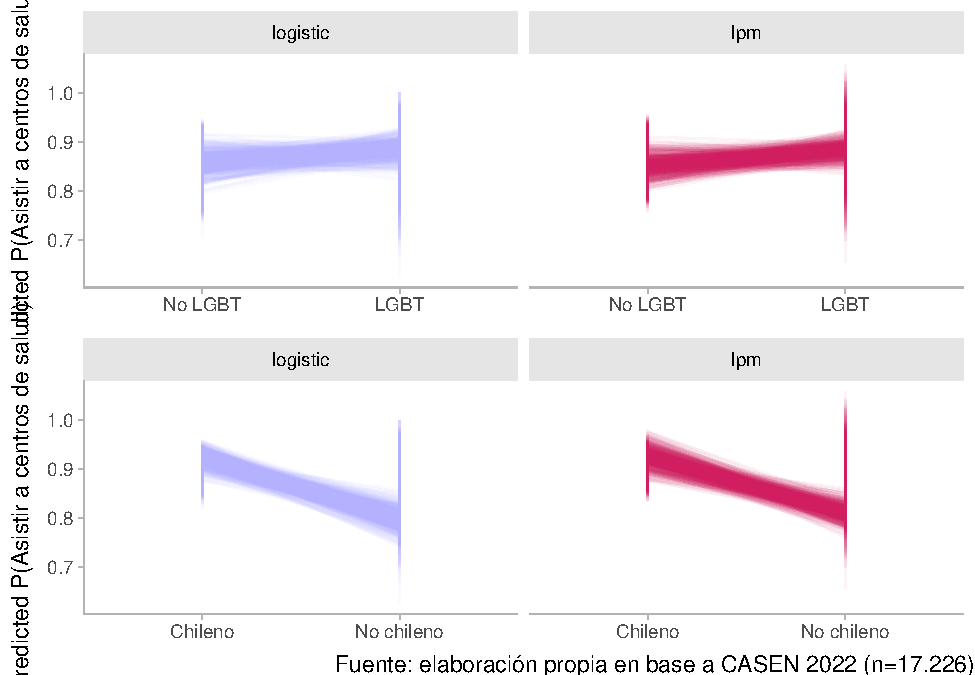
\includegraphics[width=1.05\linewidth]{trabajo_final_files/figure-latex/fig2-1} 

}

\caption{Bootstrap de coeficientes con regresión logística y modelo de probabilidad lineal}\label{fig:fig2}
\end{figure}

Con el propósito de evaluar la robustez de las estimaciones, se aplicó un análisis Bootstrap con 500 iteraciones, utilizando valores predichos obtenidos a partir de modelos logístico y de probabilidad lineal (LPM). En la Figura \ref{fig:fig2} se presentan las probabilidades promedio estimadas para el efecto de ser LGBTQ+ y la nacionalidad en ambos tipos de modelos.

Los resultados indican que las estimaciones son consistentes entre configuraciones, ya que las probabilidades estimadas mantienen patrones similares en ambas aproximaciones. En detalle, las personas LGBTQ+ presentan una probabilidad estimada consistentemente mayor de acudir a centros de salud en comparación con las personas no LGBTQ+, según ambos modelos. Asimismo, las personas de nacionalidad no chilena muestran una probabilidad estimada sistemáticamente menor de asistir a centros de salud en relación con las personas chilenas. Estos hallazgos sugieren estabilidad en los patrones observados, independientemente de la elección del modelo y de la aproximación utilizada para la estimación.

\hypertarget{conclusiones}{%
\section{Conclusiones}\label{conclusiones}}

Este estudio tenía por objetivo identificar cómo ciertos factores sociodemográficos e identitarios influyen en la asistencia a centros de salud por parte de la comunidad LGBTQ+ en Chile, tras el análisis de datos provenientes de CASEN 2022.

En relación con la hipótesis \(H_1\), que planteaba una menor probabilidad de acceso a centros de salud por parte de personas LGBTQ+ en comparación con personas heterosexuales cisgénero, los resultados indican que este efecto no es estadísticamente significativo cuando ser parte de la comunidad LGBTQ+ es considerado como único factor explicativo. Esto sugiere que, con los datos disponibles, los elementos discriminatorios que la literatura ha identificado como barreras al acceso no se manifiestan de manera directa al analizar esta población en su conjunto.

Por otro lado, respecto a la hipótesis \(H_2\), que vinculaba un menor nivel educativo con una menor probabilidad de asistencia a centros de salud, los análisis reflejan que la educación aumenta la probabilidad de acceso a estos servicios, aunque no de manera proporcional a los niveles educativos alcanzados. En términos específicos, no se observa un incremento constante en la asistencia a medida que se eleva el nivel educativo. Sin embargo, se confirma el papel de la educación como un factor relevante para explicar el acceso a la atención médica (\protect\hyperlink{ref-cabieses2020health}{Cabieses \& Oyarte, 2020}; \protect\hyperlink{ref-fletcher2009higher}{Fletcher \& Frisvold, 2009}).

Finalmente, respecto a la hipótesis \(H_3\), que proponía que las personas LGBTQ+ de nacionalidad distinta a la chilena tendrían menor probabilidad de asistir a centros de salud en comparación con las personas LGBTQ+ chilenas, los resultados muestran que, aunque la interacción entre ser LGBTQ+ y no ser chileno podría sugerir una mayor probabilidad de asistencia, esta relación no alcanza significancia estadística. Esto indica la existencia de otros factores contextuales o estructurales que podrían estar influyendo en el acceso a la atención médica para este grupo en particular.

En conclusión, los análisis realizados permiten dar cuenta que no se puede afirmar que exista un acceso diferenciado a la salud entre personas heterosexuales cisgénero y personas LGBTQ+, al menos con los datos de la encuesta CASEN 2022. Sin embargo, esto da cuenta de otros factores significativos, tal como lo son la educación y la nacionalidad y, la necesidad de aplicar enfoques interseccionales. Por lo que estas conclusiones abren las puertas para estudiar el fenómeno desde otras perspectivas, ya sean metodológicas o teóricas, con el fin de identificar los aspectos que podrían influir (o no) en el acceso a la salud de personas LGBTQ+ en Chile.

\hypertarget{referencias}{%
\section{Referencias}\label{referencias}}

\hypertarget{refs}{}
\begin{CSLReferences}{1}{0}
\leavevmode\vadjust pre{\hypertarget{ref-agresti2018introduction}{}}%
Agresti, A. (2018). \emph{An introduction to categorical data analysis}. John Wiley \& Sons.

\leavevmode\vadjust pre{\hypertarget{ref-alencar2016access}{}}%
Alencar Albuquerque, G., Lima Garcia, C. de, Silva Quirino, G. da, Alves, M. J. H., Belém, J. M., Santos Figueiredo, F. W. dos, et al.others. (2016). Access to health services by lesbian, gay, bisexual, and transgender persons: Systematic literature review. \emph{BMC International Health and Human Rights}, \emph{16}, 1--10.

\leavevmode\vadjust pre{\hypertarget{ref-cabieses2020health}{}}%
Cabieses, B., \& Oyarte, M. (2020). Health access to immigrants: Identifying gaps for social protection in health. \emph{Revista de Sa{ú}de P{ú}blica}, \emph{54}, 20.

\leavevmode\vadjust pre{\hypertarget{ref-fletcher2009higher}{}}%
Fletcher, J. M., \& Frisvold, D. E. (2009). Higher education and health investments: Does more schooling affect preventive health care use? \emph{Journal of Human Capital}, \emph{3}(2), 144--176.

\leavevmode\vadjust pre{\hypertarget{ref-hosmer2013applied}{}}%
Hosmer Jr, D. W., Lemeshow, S., \& Sturdivant, R. X. (2013). \emph{Applied logistic regression}. John Wiley \& Sons.

\leavevmode\vadjust pre{\hypertarget{ref-lampe2024health}{}}%
Lampe, N. M., Barbee, H., Tran, N. M., Bastow, S., \& McKay, T. (2024). Health disparities among lesbian, gay, bisexual, transgender, and queer older adults: A structural competency approach. \emph{The International Journal of Aging and Human Development}, \emph{98}(1), 39--55.

\leavevmode\vadjust pre{\hypertarget{ref-lim2014addressing}{}}%
Lim, F. A., Brown Jr, D. V., \& Kim, S. M. J. (2014). CE: Addressing health care disparities in the lesbian, gay, bisexual, and transgender population: A review of best practices. \emph{AJN The American Journal of Nursing}, \emph{114}(6), 24--34.

\end{CSLReferences}

\pagebreak

\hypertarget{cuxf3digo-de-r}{%
\section{Código de R}\label{cuxf3digo-de-r}}

\begin{Shaded}
\begin{Highlighting}[]
\NormalTok{knitr}\SpecialCharTok{::}\NormalTok{opts\_chunk}\SpecialCharTok{$}\FunctionTok{set}\NormalTok{(}\AttributeTok{echo =}\NormalTok{ F,}
                      \AttributeTok{warning =}\NormalTok{ F,}
                      \AttributeTok{error =}\NormalTok{ F, }
                      \AttributeTok{message =}\NormalTok{ F) }

\ControlFlowTok{if}\NormalTok{ (}\SpecialCharTok{!}\FunctionTok{require}\NormalTok{(}\StringTok{"pacman"}\NormalTok{)) }\FunctionTok{install.packages}\NormalTok{(}\StringTok{"pacman"}\NormalTok{)}

\NormalTok{pacman}\SpecialCharTok{::}\FunctionTok{p\_load}\NormalTok{(tidyverse,}
\NormalTok{               sjlabelled, }
\NormalTok{               kableExtra,}
\NormalTok{               summarytools,}
\NormalTok{               here,}
\NormalTok{               naniar,}
\NormalTok{               haven,}
\NormalTok{               texreg,}
\NormalTok{               modelr,}
\NormalTok{               ggdist,}
\NormalTok{               ggpubr,}
\NormalTok{               performance,}
\NormalTok{               DescTools)}

\FunctionTok{options}\NormalTok{(}\AttributeTok{scipen=}\DecValTok{999}\NormalTok{)}
\FunctionTok{rm}\NormalTok{(}\AttributeTok{list =} \FunctionTok{ls}\NormalTok{())}

\FunctionTok{options}\NormalTok{(}\AttributeTok{knitr.kable.NA =} \StringTok{""}\NormalTok{)}
\FunctionTok{options}\NormalTok{(}\AttributeTok{knitr.table.format=}\StringTok{"latex"}\NormalTok{)}

\FunctionTok{theme\_set}\NormalTok{(}\FunctionTok{theme\_ggdist}\NormalTok{())}
\FunctionTok{load}\NormalTok{(}\AttributeTok{file =} \FunctionTok{here}\NormalTok{(}\StringTok{"output/base\_proc.RData"}\NormalTok{))}

\NormalTok{m1 }\OtherTok{\textless{}{-}} \FunctionTok{glm}\NormalTok{(asistencia }\SpecialCharTok{\textasciitilde{}} \DecValTok{1} \SpecialCharTok{+}\NormalTok{ lgbt, }\AttributeTok{family =} \FunctionTok{binomial}\NormalTok{(}\AttributeTok{link =} \StringTok{"logit"}\NormalTok{), }
          \AttributeTok{data =}\NormalTok{ base\_proc) }

\NormalTok{m2 }\OtherTok{\textless{}{-}} \FunctionTok{glm}\NormalTok{(asistencia }\SpecialCharTok{\textasciitilde{}} \DecValTok{1} \SpecialCharTok{+}\NormalTok{ lgbt }\SpecialCharTok{+}\NormalTok{ n\_educ, }\AttributeTok{family =} \FunctionTok{binomial}\NormalTok{(}\AttributeTok{link =} \StringTok{"logit"}\NormalTok{), }
          \AttributeTok{data =}\NormalTok{ base\_proc) }

\NormalTok{m3 }\OtherTok{\textless{}{-}} \FunctionTok{glm}\NormalTok{(asistencia }\SpecialCharTok{\textasciitilde{}} \DecValTok{1} \SpecialCharTok{+}\NormalTok{ lgbt }\SpecialCharTok{+}\NormalTok{ n\_educ }\SpecialCharTok{+}\NormalTok{ nacionalidad, }\AttributeTok{family =} \FunctionTok{binomial}\NormalTok{(}\AttributeTok{link =} \StringTok{"logit"}\NormalTok{), }
          \AttributeTok{data =}\NormalTok{ base\_proc) }

\NormalTok{m4 }\OtherTok{\textless{}{-}} \FunctionTok{glm}\NormalTok{(asistencia }\SpecialCharTok{\textasciitilde{}} \DecValTok{1} \SpecialCharTok{+}\NormalTok{ lgbt }\SpecialCharTok{+}\NormalTok{ n\_educ }\SpecialCharTok{+}\NormalTok{ nacionalidad}\SpecialCharTok{*}\NormalTok{lgbt, }\AttributeTok{family =} \FunctionTok{binomial}\NormalTok{(}\AttributeTok{link =} \StringTok{"logit"}\NormalTok{), }
          \AttributeTok{data =}\NormalTok{ base\_proc) }

\NormalTok{m5 }\OtherTok{\textless{}{-}} \FunctionTok{glm}\NormalTok{(asistencia }\SpecialCharTok{\textasciitilde{}} \DecValTok{1} \SpecialCharTok{+}\NormalTok{ lgbt }\SpecialCharTok{+}\NormalTok{ n\_educ }\SpecialCharTok{+}\NormalTok{ nacionalidad}\SpecialCharTok{*}\NormalTok{lgbt }\SpecialCharTok{+} 
\NormalTok{            sexo }\SpecialCharTok{+}\NormalTok{ edad }\SpecialCharTok{+}\NormalTok{ dau }\SpecialCharTok{+}\NormalTok{ depen\_grado }\SpecialCharTok{+}\NormalTok{ disc\_wg, }\AttributeTok{family =} \FunctionTok{binomial}\NormalTok{(}\AttributeTok{link =} \StringTok{"logit"}\NormalTok{), }
          \AttributeTok{data =}\NormalTok{ base\_proc) }


\NormalTok{bs }\OtherTok{\textless{}{-}} \ControlFlowTok{function}\NormalTok{(x) \{}
\NormalTok{  df }\OtherTok{\textless{}{-}} \FunctionTok{as.data.frame}\NormalTok{(x)}
  
\NormalTok{  df }\OtherTok{\textless{}{-}}\NormalTok{ df }\SpecialCharTok{\%\textgreater{}\%}
    \FunctionTok{mutate}\NormalTok{(}
      \AttributeTok{n\_educ =} \FunctionTok{as.numeric}\NormalTok{(n\_educ),}
      \AttributeTok{disc\_wg =} \FunctionTok{as.numeric}\NormalTok{(disc\_wg),}
      \AttributeTok{depen\_grado =} \FunctionTok{as.numeric}\NormalTok{(depen\_grado),}
      \AttributeTok{dau =} \FunctionTok{as.numeric}\NormalTok{(dau),}
      \AttributeTok{nacionalidad =} \FunctionTok{as.numeric}\NormalTok{(nacionalidad),}
      \AttributeTok{sexo =} \FunctionTok{as.numeric}\NormalTok{(sexo),}
      \AttributeTok{lgbt =} \FunctionTok{as.numeric}\NormalTok{(lgbt)}
\NormalTok{    )}
  
  \CommentTok{\# Crear grid de predicción}
\NormalTok{  grid }\OtherTok{\textless{}{-}}\NormalTok{ df }\SpecialCharTok{\%\textgreater{}\%}
    \FunctionTok{data\_grid}\NormalTok{(}
      \AttributeTok{lgbt =} \FunctionTok{unique}\NormalTok{(lgbt),}
      \AttributeTok{n\_educ =}\NormalTok{ n\_educ,}
      \AttributeTok{nacionalidad =} \FunctionTok{unique}\NormalTok{(nacionalidad),}
      \AttributeTok{sexo =} \FunctionTok{unique}\NormalTok{(sexo),}
      \AttributeTok{edad =} \FunctionTok{median}\NormalTok{(edad, }\AttributeTok{na.rm =} \ConstantTok{TRUE}\NormalTok{),}
      \AttributeTok{dau =} \FunctionTok{median}\NormalTok{(dau, }\AttributeTok{na.rm =} \ConstantTok{TRUE}\NormalTok{),}
      \AttributeTok{depen\_grado =} \FunctionTok{unique}\NormalTok{(depen\_grado),}
      \AttributeTok{disc\_wg =} \FunctionTok{median}\NormalTok{(disc\_wg, }\AttributeTok{na.rm =} \ConstantTok{TRUE}\NormalTok{)}
\NormalTok{    )}
  
  \CommentTok{\# Modelos ajustados}
\NormalTok{  lpm }\OtherTok{\textless{}{-}} \FunctionTok{lm}\NormalTok{(asistencia }\SpecialCharTok{\textasciitilde{}} \DecValTok{1} \SpecialCharTok{+}\NormalTok{ lgbt }\SpecialCharTok{+}\NormalTok{ n\_educ }\SpecialCharTok{+}\NormalTok{ nacionalidad }\SpecialCharTok{*}\NormalTok{ lgbt }\SpecialCharTok{+}\NormalTok{ sexo }\SpecialCharTok{+}\NormalTok{ edad }\SpecialCharTok{+}\NormalTok{ dau }\SpecialCharTok{+}\NormalTok{ depen\_grado }\SpecialCharTok{+}\NormalTok{ disc\_wg, }\AttributeTok{data =}\NormalTok{ df)}
  
\NormalTok{  logistic }\OtherTok{\textless{}{-}} \FunctionTok{glm}\NormalTok{(asistencia }\SpecialCharTok{\textasciitilde{}} \DecValTok{1} \SpecialCharTok{+}\NormalTok{ lgbt }\SpecialCharTok{+}\NormalTok{ n\_educ }\SpecialCharTok{+}\NormalTok{ nacionalidad }\SpecialCharTok{*}\NormalTok{ lgbt }\SpecialCharTok{+}\NormalTok{ sexo }\SpecialCharTok{+}\NormalTok{ edad }\SpecialCharTok{+}\NormalTok{ dau }\SpecialCharTok{+}\NormalTok{ depen\_grado }\SpecialCharTok{+}\NormalTok{ disc\_wg, }
                  \AttributeTok{family =} \StringTok{"binomial"}\NormalTok{, }\AttributeTok{data =}\NormalTok{ df)}
  
  \CommentTok{\# Agregar predicciones al grid}
\NormalTok{  grid }\OtherTok{\textless{}{-}}\NormalTok{ grid }\SpecialCharTok{\%\textgreater{}\%}
    \FunctionTok{mutate}\NormalTok{(}
      \AttributeTok{lpm =} \FunctionTok{predict}\NormalTok{(lpm, }\AttributeTok{newdata =}\NormalTok{ grid),}
      \AttributeTok{logistic =} \FunctionTok{predict}\NormalTok{(logistic, }\AttributeTok{newdata =}\NormalTok{ grid, }\AttributeTok{type =} \StringTok{"response"}\NormalTok{)}
\NormalTok{    )}
  
  \FunctionTok{return}\NormalTok{(grid)}
\NormalTok{\}}

\NormalTok{grid }\OtherTok{\textless{}{-}}\NormalTok{ base\_proc }\SpecialCharTok{\%\textgreater{}\%} 
  \FunctionTok{bootstrap}\NormalTok{(}\DecValTok{500}\NormalTok{) }\SpecialCharTok{\%\textgreater{}\%} 
  \FunctionTok{mutate}\NormalTok{(}\AttributeTok{pred =} \FunctionTok{map}\NormalTok{(strap, }\SpecialCharTok{\textasciitilde{}} \FunctionTok{bs}\NormalTok{(.x))) }\SpecialCharTok{\%\textgreater{}\%} 
\NormalTok{  dplyr}\SpecialCharTok{::}\FunctionTok{select}\NormalTok{(.id, pred) }\SpecialCharTok{\%\textgreater{}\%} 
  \FunctionTok{unnest}\NormalTok{()}


\NormalTok{grid2 }\OtherTok{\textless{}{-}}\NormalTok{ grid }\SpecialCharTok{\%\textgreater{}\%} 
  \FunctionTok{pivot\_longer}\NormalTok{(}\AttributeTok{cols =} \SpecialCharTok{{-}}\FunctionTok{c}\NormalTok{(.id, lgbt, n\_educ, nacionalidad, sexo, }
\NormalTok{                         edad, dau, depen\_grado, disc\_wg), }
               \AttributeTok{names\_to=}\StringTok{"model"}\NormalTok{,}
               \AttributeTok{values\_to=}\StringTok{"asistencia\_hat"}\NormalTok{) }\SpecialCharTok{\%\textgreater{}\%}
  \FunctionTok{mutate}\NormalTok{(}\AttributeTok{lgbt =} \FunctionTok{if\_else}\NormalTok{(lgbt }\SpecialCharTok{==} \DecValTok{1}\NormalTok{, }\StringTok{"No LGBT"}\NormalTok{, }\StringTok{"LGBT"}\NormalTok{),}
         \AttributeTok{lgbt =} \FunctionTok{factor}\NormalTok{(lgbt, }\AttributeTok{levels =} \FunctionTok{c}\NormalTok{(}\StringTok{"No LGBT"}\NormalTok{, }\StringTok{"LGBT"}\NormalTok{)),}
         \AttributeTok{nacionalidad =} \FunctionTok{if\_else}\NormalTok{(nacionalidad }\SpecialCharTok{==} \DecValTok{1}\NormalTok{, }\StringTok{"Chileno"}\NormalTok{, }\StringTok{"No chileno"}\NormalTok{),}
\NormalTok{  ) }


\FunctionTok{library}\NormalTok{(summarytools)}

\NormalTok{dependientes }\OtherTok{\textless{}{-}}\NormalTok{ base\_proc }\SpecialCharTok{\%\textgreater{}\%} 
\NormalTok{  dplyr}\SpecialCharTok{::}\FunctionTok{select}\NormalTok{(asistencia, lgbt, n\_educ, nacionalidad, sexo, edad, dau, depen\_grado, disc\_wg) }\SpecialCharTok{\%\textgreater{}\%} 
  \FunctionTok{mutate}\NormalTok{(}\AttributeTok{asistencia =} \FunctionTok{if\_else}\NormalTok{(asistencia }\SpecialCharTok{==} \DecValTok{1}\NormalTok{, }\StringTok{"Asiste"}\NormalTok{, }\StringTok{"No asiste"}\NormalTok{),}
         \AttributeTok{asistencia =} \FunctionTok{factor}\NormalTok{(asistencia, }\AttributeTok{levels =} \FunctionTok{c}\NormalTok{(}\StringTok{"No asiste"}\NormalTok{, }\StringTok{"Asiste"}\NormalTok{)))}


\NormalTok{dependientes}\SpecialCharTok{$}\NormalTok{asistencia }\OtherTok{\textless{}{-}}\NormalTok{ sjlabelled}\SpecialCharTok{::}\FunctionTok{set\_label}\NormalTok{(dependientes}\SpecialCharTok{$}\NormalTok{asistencia, }\StringTok{"Asistencia centros de salud"}\NormalTok{)}

\NormalTok{dependientes}\SpecialCharTok{$}\NormalTok{lgbt }\OtherTok{\textless{}{-}}\NormalTok{ sjlabelled}\SpecialCharTok{::}\FunctionTok{set\_label}\NormalTok{(dependientes}\SpecialCharTok{$}\NormalTok{lgbt, }\StringTok{"LGBTQ+"}\NormalTok{)}

\NormalTok{dependientes}\SpecialCharTok{$}\NormalTok{n\_educ }\OtherTok{\textless{}{-}}\NormalTok{ sjlabelled}\SpecialCharTok{::}\FunctionTok{set\_label}\NormalTok{(dependientes}\SpecialCharTok{$}\NormalTok{n\_educ, }\StringTok{"Nivel educacional"}\NormalTok{)}

\NormalTok{dependientes}\SpecialCharTok{$}\NormalTok{nacionalidad }\OtherTok{\textless{}{-}}\NormalTok{ sjlabelled}\SpecialCharTok{::}\FunctionTok{set\_label}\NormalTok{(dependientes}\SpecialCharTok{$}\NormalTok{nacionalidad, }\StringTok{"Nacionalidad"}\NormalTok{)}

\NormalTok{dependientes}\SpecialCharTok{$}\NormalTok{sexo }\OtherTok{\textless{}{-}}\NormalTok{ sjlabelled}\SpecialCharTok{::}\FunctionTok{set\_label}\NormalTok{(dependientes}\SpecialCharTok{$}\NormalTok{sexo, }\StringTok{"Sexo"}\NormalTok{)}


\NormalTok{dependientes}\SpecialCharTok{$}\NormalTok{disc\_wg }\OtherTok{\textless{}{-}}\NormalTok{ sjlabelled}\SpecialCharTok{::}\FunctionTok{set\_label}\NormalTok{(dependientes}\SpecialCharTok{$}\NormalTok{disc\_wg, }\StringTok{"Discapacidad"}\NormalTok{)}

\NormalTok{dependientes}\SpecialCharTok{$}\NormalTok{depen\_grado }\OtherTok{\textless{}{-}}\NormalTok{ sjlabelled}\SpecialCharTok{::}\FunctionTok{set\_label}\NormalTok{(dependientes}\SpecialCharTok{$}\NormalTok{depen\_grado, }\StringTok{"Grado de dependencia"}\NormalTok{)}

\NormalTok{df}\OtherTok{\textless{}{-}}\FunctionTok{dfSummary}\NormalTok{(dependientes,}
               \AttributeTok{plain.ascii =} \ConstantTok{FALSE}\NormalTok{,}
               \AttributeTok{style =} \StringTok{"multiline"}\NormalTok{,}
               \AttributeTok{tmp.img.dir =} \StringTok{"/tmp"}\NormalTok{,}
               \AttributeTok{graph.magnif =} \FloatTok{0.75}\NormalTok{,}
               \AttributeTok{headings =}\NormalTok{ F,  }\CommentTok{\# encabezado}
               \AttributeTok{varnumbers =}\NormalTok{ F, }\CommentTok{\# num variable}
               \AttributeTok{labels.col =}\NormalTok{ T, }\CommentTok{\# etiquetas}
               \AttributeTok{na.col =}\NormalTok{ F,    }\CommentTok{\# missing}
               \AttributeTok{graph.col =}\NormalTok{ F, }\CommentTok{\# plot}
               \AttributeTok{valid.col =}\NormalTok{ T, }\CommentTok{\# n valido}
               \AttributeTok{col.widths =} \FunctionTok{c}\NormalTok{(}\DecValTok{30}\NormalTok{,}\DecValTok{10}\NormalTok{,}\DecValTok{10}\NormalTok{,}\DecValTok{10}\NormalTok{))}

\NormalTok{df}\SpecialCharTok{$}\NormalTok{Variable }\OtherTok{\textless{}{-}} \ConstantTok{NULL} \CommentTok{\# delete variable column}

\FunctionTok{print}\NormalTok{(df)}


\NormalTok{ccoef }\OtherTok{\textless{}{-}} \FunctionTok{list}\NormalTok{(}
  \StringTok{"(Intercept)"} \OtherTok{=} \StringTok{"Intercepto"}\NormalTok{,}
   \AttributeTok{lgbtLGBT  =} \StringTok{"LGBT (Ref.= No LGBT)"}\NormalTok{,}
  \StringTok{"n\_educBásica Incompleta"} \OtherTok{=} \StringTok{"Básica incompleta"}\NormalTok{,}
  \StringTok{"n\_educBásica Completa"} \OtherTok{=} \StringTok{"Básica completa"}\NormalTok{,}
  \StringTok{"n\_educMedia Incompleta"} \OtherTok{=} \StringTok{"Media incompleta"}\NormalTok{,   }
  \StringTok{"n\_educMedia Completa"}  \OtherTok{=} \StringTok{"Media completa"}\NormalTok{,}
  \StringTok{"n\_educSuperior Incompleta"} \OtherTok{=} \StringTok{"Superior incompleta"}\NormalTok{,      }
  \StringTok{"n\_educSuperior Completa"} \OtherTok{=} \StringTok{"Superior completa"}\NormalTok{,}
  \StringTok{"nacionalidadNo chileno"}  \OtherTok{=} \StringTok{"Nacionalidad no chilena (Ref.= Chilena)"}\NormalTok{,         }
  \StringTok{"lgbtLGBT:nacionalidadNo chileno"} \OtherTok{=} \StringTok{"LGBT x Nacionalidad no chilena"}\NormalTok{,}
  \StringTok{"sexoMujer"} \OtherTok{=} \StringTok{"Mujer (Ref. = Hombre)"}\NormalTok{,}
  \AttributeTok{edad =} \StringTok{"Edad"}\NormalTok{,}
  \AttributeTok{dau =} \StringTok{"Ingresos"}\NormalTok{,}
  \StringTok{"depen\_gradoDependencia leve"} \OtherTok{=} \StringTok{"Dependencia leve"}\NormalTok{, }
  \StringTok{"depen\_gradoDependencia moderada"} \OtherTok{=} \StringTok{"Dependencia moderadada"}\NormalTok{,}
  \StringTok{"depen\_gradoDependencia severa"} \OtherTok{=} \StringTok{"Dependencia severa"}\NormalTok{,        }
  \StringTok{"disc\_wgCon discapacidad"} \OtherTok{=} \StringTok{"Tiene discapacidad (Ref. = No tiene)"}
\NormalTok{  )}

\NormalTok{texreg}\SpecialCharTok{::}\FunctionTok{texreg}\NormalTok{(}\FunctionTok{list}\NormalTok{(m1, m2, m3, m4, m5),}
               \AttributeTok{custom.model.names =} \FunctionTok{c}\NormalTok{(}\StringTok{"Modelo 1"}\NormalTok{, }\StringTok{"Modelo 2"}\NormalTok{, }\StringTok{"Modelo 3"}\NormalTok{, }\StringTok{"Modelo 4"}\NormalTok{, }\StringTok{"Modelo 5"}\NormalTok{),}
               \AttributeTok{caption =} \FunctionTok{paste}\NormalTok{(}\StringTok{"(}\SpecialCharTok{\textbackslash{}\textbackslash{}}\StringTok{\#tab:table2)"}\NormalTok{,}\StringTok{"Modelos de regresión logística para la probabilidad de asistir a centros de salud"}\NormalTok{),}
               \AttributeTok{stars =} \FunctionTok{c}\NormalTok{(}\FloatTok{0.05}\NormalTok{, }\FloatTok{0.01}\NormalTok{, }\FloatTok{0.001}\NormalTok{),}
               \AttributeTok{custom.coef.map =}\NormalTok{ ccoef,}
               \AttributeTok{groups =} \FunctionTok{list}\NormalTok{(}\StringTok{"Nivel educacional (Ref.= Sin Ed. Formal)"} \OtherTok{=} \DecValTok{3}\SpecialCharTok{:}\DecValTok{8}\NormalTok{,}
                            \StringTok{"Grado dependencia (Ref. = Sin dependencia)"} \OtherTok{=} \DecValTok{13}\SpecialCharTok{:}\DecValTok{15}\NormalTok{),}
               \AttributeTok{custom.note =} \StringTok{"}\SpecialCharTok{\textbackslash{}\textbackslash{}}\StringTok{item Nota: Celdas contienen coeficientes de regresión con errores estándares entre paréntesis. \%stars. }\SpecialCharTok{\textbackslash{}\textbackslash{}\textbackslash{}\textbackslash{}}\StringTok{ }\SpecialCharTok{\textbackslash{}\textbackslash{}}\StringTok{item Fuente: elaboración propia con datos de CASEN 2022 (n = 17.226)"}\NormalTok{,}
               \AttributeTok{threeparttable =}\NormalTok{ T,}
               \AttributeTok{leading.zero =}\NormalTok{ T,}
               \AttributeTok{float.pos =} \StringTok{"h!"}\NormalTok{,}
               \AttributeTok{use.packages =}\NormalTok{ F,}
               \AttributeTok{booktabs =}\NormalTok{ T,}
               \AttributeTok{scalebox =} \FloatTok{0.8}\NormalTok{)}


\NormalTok{marginaleffects}\SpecialCharTok{::}\FunctionTok{plot\_slopes}\NormalTok{(m4, }
                             \AttributeTok{variables =} \StringTok{"lgbt"}\NormalTok{, }
                             \AttributeTok{condition =} \StringTok{"nacionalidad"}\NormalTok{, }
                             \AttributeTok{conf\_level =} \FloatTok{0.95}\NormalTok{, }
                             \AttributeTok{re.form =} \ConstantTok{NA}\NormalTok{) }\SpecialCharTok{+}
  \FunctionTok{geom\_hline}\NormalTok{(}\AttributeTok{yintercept =} \DecValTok{0}\NormalTok{, }
             \AttributeTok{color =} \StringTok{"red"}\NormalTok{, }
             \AttributeTok{linetype =} \StringTok{"dashed"}\NormalTok{) }\SpecialCharTok{+}
  \FunctionTok{labs}\NormalTok{(}\AttributeTok{y =} \StringTok{"Efecto marginal de LGBTQ+"}\NormalTok{,}
       \AttributeTok{x =} \StringTok{"Nacionalidad"}\NormalTok{,}
      \AttributeTok{caption=} \StringTok{"Fuente: elaboración propia con datos de CASEN 2022 (n = 17.226)"}\NormalTok{,}
       \AttributeTok{title =} \ConstantTok{NULL}\NormalTok{)}


\NormalTok{aic }\OtherTok{\textless{}{-}} \FunctionTok{AIC}\NormalTok{(m5)}
\NormalTok{bic }\OtherTok{\textless{}{-}} \FunctionTok{BIC}\NormalTok{(m5)}
\NormalTok{r2\_mcfadden }\OtherTok{\textless{}{-}} \FunctionTok{as.numeric}\NormalTok{(}\FunctionTok{PseudoR2}\NormalTok{(m5, }\AttributeTok{which =} \StringTok{"McFadden"}\NormalTok{))}
\NormalTok{pcp }\OtherTok{\textless{}{-}}\NormalTok{ performance}\SpecialCharTok{::}\FunctionTok{performance}\NormalTok{(m5)  }\SpecialCharTok{\%\textgreater{}\%} 
  \FunctionTok{as\_tibble}\NormalTok{() }\SpecialCharTok{\%\textgreater{}\%} 
  \FunctionTok{select}\NormalTok{(PCP) }\SpecialCharTok{\%\textgreater{}\%} 
  \FunctionTok{pull}\NormalTok{()}
  

\NormalTok{results\_table }\OtherTok{\textless{}{-}} \FunctionTok{data.frame}\NormalTok{(}
  \AttributeTok{Indicador =} \FunctionTok{c}\NormalTok{(}\StringTok{"AIC"}\NormalTok{, }\StringTok{"BIC"}\NormalTok{, }\StringTok{"R2 McFadden"}\NormalTok{, }\StringTok{"PCP (\%)"}\NormalTok{),}
  \AttributeTok{Valor =} \FunctionTok{c}\NormalTok{(aic, bic, r2\_mcfadden, pcp}\SpecialCharTok{*}\DecValTok{100}\NormalTok{)}
\NormalTok{)}

\NormalTok{results\_table }\SpecialCharTok{\%\textgreater{}\%} 
\NormalTok{ kableExtra}\SpecialCharTok{::}\FunctionTok{kable}\NormalTok{(}\AttributeTok{format =} \StringTok{"latex"}\NormalTok{, }
                    \AttributeTok{col.names =} \FunctionTok{c}\NormalTok{(}\StringTok{"Indicador"}\NormalTok{, }\StringTok{"Valor"}\NormalTok{),}
                    \AttributeTok{row.names =}\NormalTok{ F,}
                    \AttributeTok{booktabs =}\NormalTok{ T, }\AttributeTok{align =} \StringTok{\textquotesingle{}l\textquotesingle{}}\NormalTok{,}
                    \AttributeTok{caption =} \FunctionTok{paste}\NormalTok{(}\StringTok{"(}\SpecialCharTok{\textbackslash{}\textbackslash{}}\StringTok{\#tab:table3)"}\NormalTok{,}\StringTok{"Estadísticos de bondad de ajuste Modelo 5"}\NormalTok{)) }\SpecialCharTok{\%\textgreater{}\%} 
\NormalTok{  kableExtra}\SpecialCharTok{::}\FunctionTok{kable\_styling}\NormalTok{(}\AttributeTok{latex\_options =} \StringTok{"hold\_position"}\NormalTok{, }
                            \AttributeTok{position =} \StringTok{"center"}\NormalTok{) }\SpecialCharTok{\%\textgreater{}\%}
\NormalTok{  kableExtra}\SpecialCharTok{::}\FunctionTok{kable\_styling}\NormalTok{(}\AttributeTok{bootstrap\_options =} \FunctionTok{c}\NormalTok{(}\StringTok{"striped"}\NormalTok{, }\StringTok{"hover"}\NormalTok{, }\StringTok{"condensed"}\NormalTok{, }\StringTok{"responsive"}\NormalTok{), }\AttributeTok{full\_width =}\NormalTok{ F) }\SpecialCharTok{\%\textgreater{}\%} 
\NormalTok{  kableExtra}\SpecialCharTok{::}\FunctionTok{column\_spec}\NormalTok{(}\DecValTok{1}\NormalTok{, }\AttributeTok{width =} \StringTok{"8cm"}\NormalTok{) }\SpecialCharTok{\%\textgreater{}\%}
\NormalTok{  kableExtra}\SpecialCharTok{::}\FunctionTok{row\_spec}\NormalTok{(}\DecValTok{0}\NormalTok{, }\AttributeTok{bold =}\NormalTok{ T)}


\NormalTok{p1 }\OtherTok{\textless{}{-}}\NormalTok{ grid2 }\SpecialCharTok{\%\textgreater{}\%} 
  \FunctionTok{ggplot}\NormalTok{(}\FunctionTok{aes}\NormalTok{(}\AttributeTok{x=}\NormalTok{lgbt,}\AttributeTok{y=}\NormalTok{asistencia\_hat, }\AttributeTok{group=}\FunctionTok{interaction}\NormalTok{(.id), }\AttributeTok{colour=}\NormalTok{model)) }\SpecialCharTok{+}
  \FunctionTok{geom\_line}\NormalTok{(}\AttributeTok{alpha=}\NormalTok{.}\DecValTok{05}\NormalTok{) }\SpecialCharTok{+}
  \FunctionTok{scale\_color\_manual}\NormalTok{(}\AttributeTok{values =} \FunctionTok{c}\NormalTok{(}\StringTok{"\#aba8fa"}\NormalTok{, }\StringTok{"\#c71558"}\NormalTok{)) }\SpecialCharTok{+}
  \FunctionTok{facet\_wrap}\NormalTok{(}\SpecialCharTok{\textasciitilde{}}\NormalTok{model) }\SpecialCharTok{+}
  \FunctionTok{labs}\NormalTok{(}\AttributeTok{x =} \ConstantTok{NULL}\NormalTok{,}
       \AttributeTok{y =} \StringTok{"Predicted P(Asistir a centros de salud)"}\NormalTok{) }\SpecialCharTok{+}
  \FunctionTok{theme\_ggdist}\NormalTok{() }\SpecialCharTok{+}
  \FunctionTok{theme}\NormalTok{(}\AttributeTok{legend.position =} \StringTok{"none"}\NormalTok{)}


\NormalTok{p2 }\OtherTok{\textless{}{-}}\NormalTok{ grid2 }\SpecialCharTok{\%\textgreater{}\%} 
  \FunctionTok{ggplot}\NormalTok{(}\FunctionTok{aes}\NormalTok{(}\AttributeTok{x=}\NormalTok{nacionalidad,}\AttributeTok{y=}\NormalTok{asistencia\_hat, }\AttributeTok{group=}\FunctionTok{interaction}\NormalTok{(.id), }\AttributeTok{colour=}\NormalTok{model)) }\SpecialCharTok{+}
  \FunctionTok{geom\_line}\NormalTok{(}\AttributeTok{alpha=}\NormalTok{.}\DecValTok{05}\NormalTok{) }\SpecialCharTok{+}
  \FunctionTok{scale\_color\_manual}\NormalTok{(}\AttributeTok{values =} \FunctionTok{c}\NormalTok{(}\StringTok{"\#aba8fa"}\NormalTok{, }\StringTok{"\#c71558"}\NormalTok{)) }\SpecialCharTok{+}
  \FunctionTok{facet\_wrap}\NormalTok{(}\SpecialCharTok{\textasciitilde{}}\NormalTok{model) }\SpecialCharTok{+}
  \FunctionTok{labs}\NormalTok{(}\AttributeTok{x =} \ConstantTok{NULL}\NormalTok{,}
       \AttributeTok{y =} \StringTok{"Predicted P(Asistir a centros de salud)"}\NormalTok{) }\SpecialCharTok{+}
  \FunctionTok{theme\_ggdist}\NormalTok{() }\SpecialCharTok{+}
  \FunctionTok{theme}\NormalTok{(}\AttributeTok{legend.position =} \StringTok{"none"}\NormalTok{)}
  
\FunctionTok{ggarrange}\NormalTok{(p1, p2, }
          \AttributeTok{ncol =} \DecValTok{1}\NormalTok{) }\SpecialCharTok{+}
  \FunctionTok{theme}\NormalTok{(}\AttributeTok{plot.caption =} \FunctionTok{element\_text}\NormalTok{(}\AttributeTok{hjust =} \DecValTok{1}\NormalTok{, }\AttributeTok{size =} \DecValTok{11}\NormalTok{)) }\SpecialCharTok{+}
  \FunctionTok{labs}\NormalTok{(}\AttributeTok{caption =} \StringTok{"Fuente: elaboración propia en base a CASEN 2022 (n=17.226)"}\NormalTok{)}
\end{Highlighting}
\end{Shaded}


\end{document}
